\chapter{はじめに}
\label{ch:introduction}
現代において,ニュースを始めとする情報入手と拡散が簡単にできるSNS(ソーシャルメディア)は生活の重要な一部となった.
SNSは現在$\mathbb{X}$(旧Twitter、以後Twitterと表記)をはじめFacebook, Instagram, YouTube, TikTokと多くのプラットフォーム上に多様な情報が拡散されている。
しかし、中には信憑性に乏しい情報が含まれており,特に悪意によって読者を騙して誤った風説を流布するために作られた情報であるフェイクニュース及び偽情報が社会問題となっている.
%フェイクニュースの国際的にコンセンサスが取れた定義はないが,``Fake news''という語は既に19世紀の文献に使われているという報告が英英辞典出版会社であるMerriam-Webstarから指摘されている\cite{merriam-webster}.
%また同時に辞書に載せない理由としてフェイクニュースという語が自明の意味をもつためとも指摘されている\cite{merriam-webster}.
本研究はこれまでの研究\cite{Shu:2017:FND:3137597.3137600,Ruchansky:2017:CHD:3132847.3132877,Wang:2018:EEA:3219819.3219903}に倣い,意図的に作成され,明確に誤りであると確認できる情報を偽情報と定義し、検出対象とする.

偽情報の実例として,近年は新型コロナウイルス感染症(COVID-19)にまつわる誤った風説がSNS上で広く流布された.
WHO事務局長はこの問題を``インフォデミック''と呼び,偽情報はウイルスそのものよりも早く簡単に拡散されると警戒を呼びかけている\cite{ZAROCOSTAS2020676}.
また,偽情報によってオンラインで誤った風説が広がった結果,オフラインの出来事へ大きな影響を与えたこともある.
英国では「第5世代移動通信システム(5G)が健康被害をもたらし,新型コロナウイルス感染症蔓延に寄与している」という偽情報に基づく陰謀論が流布された結果,基地局の設備が壊された\cite{waterson_hern_2020}ほかに作業員が暴行や暴言を受けた\cite{hern_2020}.
以上より,偽情報の拡散によって読者が事実に基づく正しいニュースへのアクセスが難しくなるため、政情不安・暴力・テロリズムを引き起こすことで民主主義の根幹を揺るがす深刻な問題であると世界経済フォーラムの年次報告書は指摘している \cite{mclennan2024global}.

現在,偽情報検出に向けて有識者が事実関係を確認して結果を公表するファクトチェックが行われている.
\begin{figure}[p]
    \centering
    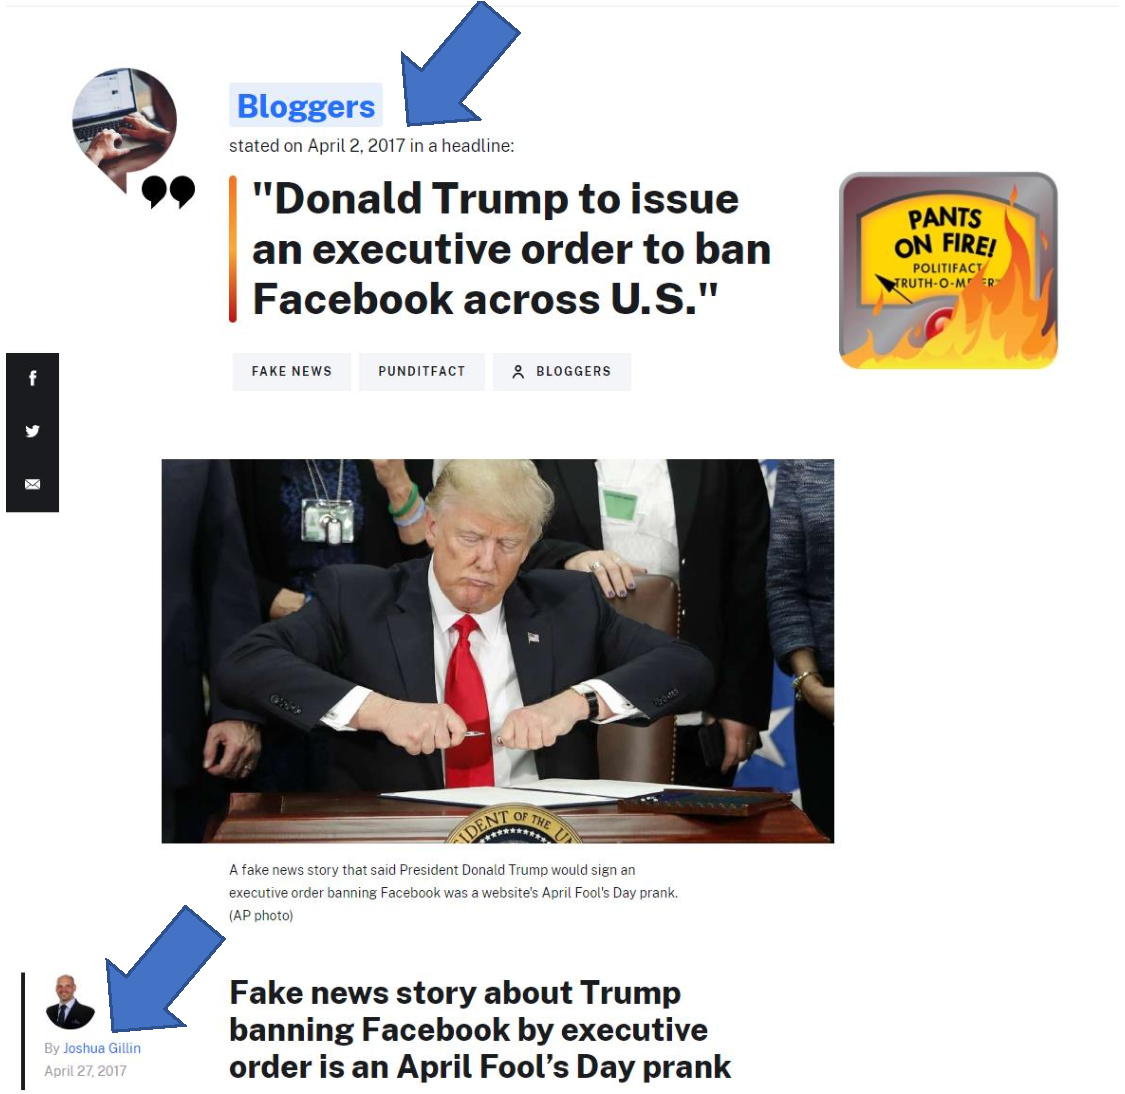
\includegraphics[width=0.8\linewidth]{figures/fact-check.pdf}
    \caption{
        北米で行われたファクトチェックの一例.
        % この情報はエイプリルフールで投稿された虚偽情報としている.
        青矢印は元情報の投稿日時とファクトチェック結果投稿日時を示し,両者には25日もの間隔がある.
        }
    \label{fig:example}
\end{figure}

図\ref{fig:example}はファクトチェックの一例である\cite{gillin_2017}.
この実例のように,ファクトチェックは属人的な作業であることに加えて結果公表まで時間がかかるため,
ファクトチェック結果は偽情報そのものに比べて拡散されにくい.
このため,機械学習によって偽情報を自動で検出する研究が行われている.

自動検出にあたって困難な点として,偽情報は人々を騙すために巧妙なつくりをしていることが挙げられる.
このため,単純なルールベース手法による検出は難しい.
また、現在偽情報をとりまく状況は変化しており、文章に限らず画像・動画・音声など多様な媒体で発信されるようになった。
\cref{tab:modality}は4種の媒体別の流布頻度と既存研究から現在の状況を示している。
文章・画像は流布される頻度が最も高い一方で多くの既存研究が提案されている。
一方で動画は流布される頻度が上昇傾向にあるが、動画の多くは拡散の早い段階で虚偽と検証されて拡散に歯止めがかかりやすい上に、
動画及び映像を検出対象とした研究も多数提案されている。
しかしながら音声は流布される頻度が動画以上に激しい上昇傾向にある。
その上、既存研究の多くはSNSではなく生体認証から発展させた形であるため、現在の偽情報を取り巻く状況への合致が求められている。
% 

\begin{landscape}
\begin{table}[p]
    \centering
    \begin{tabular}{l|c|c|c} \hline
       媒体 & 流布頻度 & 既存研究 & 概説\\ \hline\hline
       文章 & 多い & \cite{yanagi2021classifying,10.1145/3292500.3330935} & 噂を含めれば最も高い頻度で流布されている一方、検出を目指す既存研究も多い \\
       画像 & 多い & \cite{Wang:2018:EEA:3219819.3219903,8919302} & 記事文章と関係ない画像の使用や合成・生成画像を検出対象とした研究が多い \\
       動画 & 緩やかな増加 & \cite{8683164,8668407} & 増加傾向にあるが、その多くは早い段階で虚偽として注意喚起がなされている \\
       \multirow{2}{*}{音声} & \multirow{2}{*}{急激に増加\cite{cox_2023}} & \multirow{2}{*}{\cite{yamagishi21_asvspoof}} & %動画の構成要素としての音声や
       激しい増加に個別の検証が追いついていおらず、\\
       & & & 自動検出する研究もSNSを想定した形は限られる \\ \hline
    \end{tabular}
    \caption{偽情報の媒体別の流布状況及び既存研究に準拠した状況の概説}
    \label{tab:modality}
\end{table}
\end{landscape}

% 媒体を問わず唐突?
本研究では、現状AIによる生成技術の発展に検出が追いついていない偽情報を話す音声の検出も視野に入れ、
媒体を問わず広く検出が行える手法と音声に特化した手法の2種類を提案する。
これにより、急速に変化する偽情報を取り巻く事情に多面的に対処が可能となる。

先行研究では、検出性能の向上において,記事そのものがもつ情報に加えてソーシャルメディア上での反響を示すソーシャルコンテキスト(リツイート・いいね・リプライなど)
を考慮する有効性が指摘されている\cite{Guo:2018:RDH:3269206.3271709}.
しかしながら,ソーシャルコンテキストはユーザの拡散によって生まれるため,この場合も早期の検出には向かない.
これに対して,ニュースに対してソーシャルメディア上で寄せられるコメントで発生しやすい単語を,条件付き変分オートエンコーダ(CVAE)で生成する手法も提案されている\cite{ijcai2018-533}.
この手法は,記事から確率分布とラベルを元に隠し変数を介して生成を行っている.

本研究では、記事と実際に記事に寄せられたコメントから信憑性の学習を行い,記事と限られた数のコメントから別のコメントを予測させた上で真偽を判断するモデルを提案する。
このモデルは,偽情報そのものを生成するモデル\cite{DBLP:journals/corr/abs-1905-12616}を拡張する形で実装することでコメントの生成を実現する.
学習では記事と実際に記事に寄せられたコメントを3件,更に真偽ラベルを入力するが,テスト時は記事に加えて実際に寄せられたコメントは2件に制限し,真偽ラベルは入力しない.

我々は提案モデルの検出性能を実際に投稿された情報をもつデータセットによって検証した結果,生成コメントを加えた影響でより多くの偽情報を検出することに成功した.
また生成コメントの有無で検出傾向を調べたところ,生成コメントの追加によってFakeをRealと誤認する事例が減少したことが確認された.

一方で、近年さらに偽情報の検出を困難にしている点として、音声や動画といったニュース媒体の多様化が挙げられる。
中でも偽情報を話すなりすまし偽音声や偽動画も偽情報問題と同じく、センセーショナルさを持つがゆえにソーシャルメディアで急速に拡散される危険性を持っている。
広く拡散された偽情報動画の例として、2022年にウクライナのゼレンスキー大統領になりすましたものが挙げられる。
\cref{fig:zelensky}はその動画と本人の写真を並べたものである。
\begin{figure}  %TODO: かえる
    \centering
    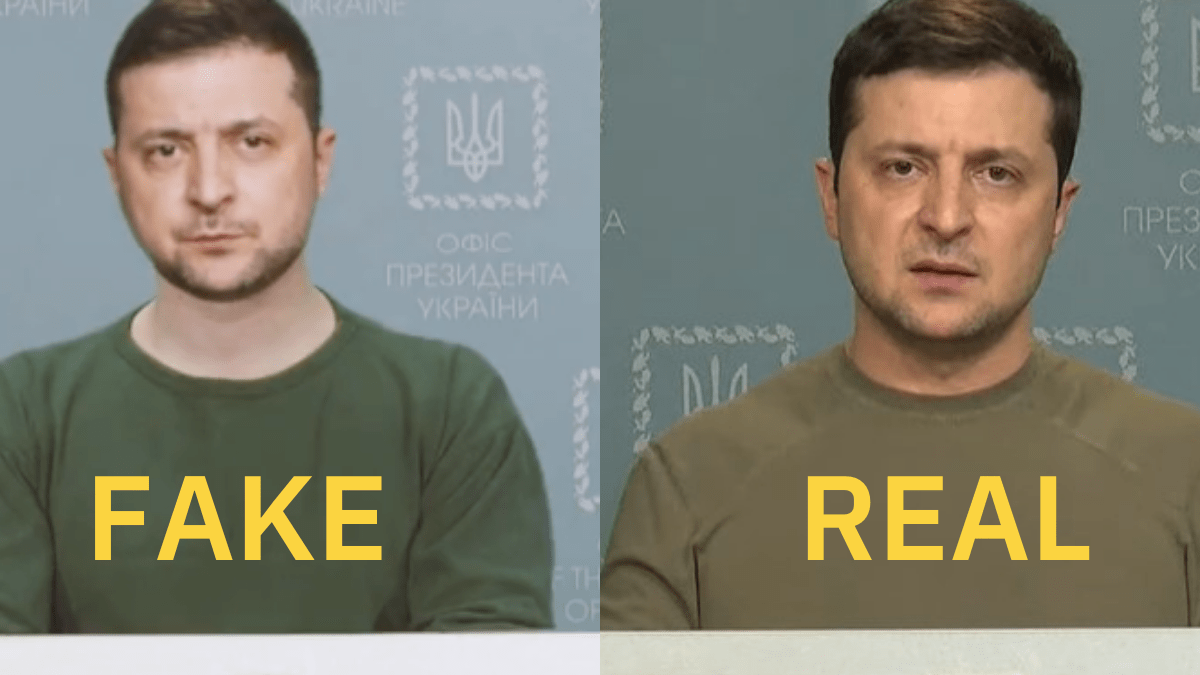
\includegraphics[width=0.45\textwidth]{figures/zelensky.png}
    \caption{ウクライナのゼレンスキー大統領が動画で投降を呼びかける音声付きディープフェイク動画 \cite{evon_2022}.}
    \label{fig:zelensky}
\end{figure}
この動画は武器を捨てて投稿するよう呼びかけていたが、事実確認(ファクトチェック)によって虚偽と認められた \cite{Staff_2020}。
他にもアメリカのペロシ前下院議長になりすました動画は2023年に新たに投稿されており、ロイター通信によって虚偽と確認されている \cite{Check_2023}。
このようなディープフェイク映像の対策として、映像そのものの分析 \cite{8683164}やメディアの出自 \cite{8668407}から信憑性を評価して検出を目指した研究が提案されている。
なりすまし音声による虚偽の主張が盛んに投稿された事例もある。
2023年初頭に公開された音声生成AIによって有名人になりすました偽情報がSNSに投稿され、中には人種及び性的少数者に対する差別的なものも含まれていた \cite{cox_2023}。
容易に特定の人物を模した音声を合成する手法には、文章を入力に出力音声を得るText-To-Speech(文章読み上げ、TTS) \cite{klatt1987review}と、他人の音声を入力に対象人物の音声に変換するVoice Conversion(音声変換、VC) \cite{661472}の2種類がある。
\cref{fig:vctts}は2種類の手法によるなりすまし事例を示す模式図である。
本研究では、TTSによって生成された音声を検出対象とした。
これは少ないコストで大量に合成音声を用意できる点から、すべてを人手での確認することが難しく自動で検出する必要が強いためである。
\begin{figure}[p]
\centering
  \begin{minipage}[b]{0.8\linewidth}
    \centering
    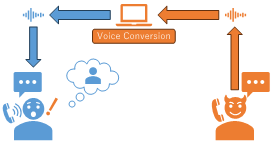
\includegraphics[keepaspectratio, width=0.8\linewidth]{figures/vc.png}
    \subcaption{Voice Conversionによる場合。}
  \end{minipage}
  \begin{minipage}[b]{0.8\linewidth}
    \centering
    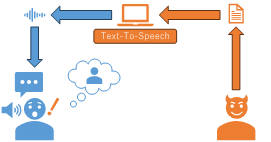
\includegraphics[keepaspectratio, width=0.8\linewidth]{figures/tts.png}
    \subcaption{Text-To-Speechによる場合。}
  \end{minipage}
  \caption{偽音声によるなりすましを示す模式図。(a)のVoice Conversionでは攻撃者の音声が入力であり、(b)のText-To-Speechでは文章が入力であるため攻撃者の音声は含まれない。}
  \label{fig:vctts}
\end{figure}

なりすまし音声による偽情報に対して現在行われている検出手法の多くは、生体認証システムに対する攻撃を念頭に置いたものが中心である。この代表としてASVspoof \cite{7858696,kinnunen17_interspeech,todisco19_interspeech}という共有タスクが2015年から隔年で開催されている。
以前は電話回線や録音再生を想定したシナリオに限られていたが2021年の開催で初めてSNS上での投稿を想定したシナリオが追加された \cite{yamagishi21_asvspoof}。
この取り組みでは同じ文章を人間が読み上げたものと合成音声による2種へ分類を行うモデルを募っている。
読み上げる内容は同じであるため、参加手法は音声波形を直接入力として扱っている\cite{jung20c_interspeech,9746213}。
ASVspoof以外では入力音声から声道を再構築して合成か本物かを判断する手法も提案された \cite{280020}。

これら手法が共通して抱える問題点として、合成側の技術進歩が著しい上に検出手法は攻撃側も利用できるため、生成性能の向上による検出性能の低下が激しい点が挙げられる。
実際に2021年に開催されたASVspoofでは、学習用データは2019年開催のものを流用し、手法の評価には2019年以降に提案された新型生成手法によって生成された音声を使用した。
その結果、学習時の分類性能に比べて評価時の性能が大きく劣化する傾向がみられた \cite{yamagishi21_asvspoof,yu_icmece}。
一方で、問題を起こすなりすまし音声は虚偽の主張を行うものが多いため、
音声内で話される内容を含めて信憑性を評価することは有効と考えられるが、そのような手法はみられない。
今後合成音声の精巧化が進むと、波形そのものの自然さ/クオリティの検証と同時に発話内容そのものを検証する重要性が強まることが予想されている \cite{10208955}。

そこで本研究では、発話内容も考慮に入れてなりすまし音声による偽情報を自動で検出するモデルの構築を目指した。
具体的には、入力音声そのものが合成あるいは本物であるかと、主張内容は疑わしいかそうでないかという2点の観点からなりすまし音声による偽情報の検出を行う。
検出対象として、既存の偽情報データセット \cite{10.1145/3477495.3531744}が持つTwitterツイート群から、
直近提案された中で著名なTTS手法であるVITS \cite{pmlr-v139-kim21f}によって生成した音声データを用意した。
本研究の目的は既存の手法に新たに発話内容を考慮する重要性を示すものであるため、
入力音声そのものを直接入力として扱う手法は既存のものを使用した。
発話内容の考慮には、偽情報データセットの各ツイートから得た文章埋め込みをニューラルネットワークを介して信憑性を評価する独自モデルを用意した。
この結果、音声波形のみを扱う手法では、直近の合成音声手法による偽音声を正確に検出できなかった点に対して,
文章埋め込みに基づく真偽二値分類に由来する入力を追加することによって、検出性能が改善した.


%全体の流れ
本論文の構成は次の通りである.
\cref{ch:background}では,本研究が扱う偽情報に関する背景を実例を交えて記述する.
\cref{ch:rel_res}では,本研究と関連のある研究や取り組みを紹介する.
\cref{ch:gen_com}では,第一の手法として記事に対してコメントを生成して検出を補助する形式及び実験を説明する。
\cref{ch:spc_cnt}では,第ニの手法として発話音声も加味したなりすまし偽音声検出を行う形式及び実験を説明する.
\cref{ch:discussion}では,\cref{ch:gen_com}と\cref{ch:spc_cnt}の実験を併せた全体の考察とともに、手法や結果から浮かび上がった課題についても指摘する.
\cref{ch:conclusion}では,本論文をまとめるとともに,実用化を含めた今後の発展形についていくつかの展開を記載している.